\RequirePackage{fix-cm}
\documentclass[11pt,a4paper]{article}
\usepackage[margin=2.5cm]{geometry}
\usepackage[T1]{fontenc}
\usepackage[utf8]{inputenc}

\usepackage{cite}
\usepackage{amsmath,amssymb,amsfonts}
\usepackage{algorithm}
\usepackage{algpseudocode}
\usepackage{graphicx}
\usepackage[section]{placeins}
\renewcommand{\topfraction}{0.9}
\renewcommand{\bottomfraction}{0.8}
\renewcommand{\textfraction}{0.08}
\renewcommand{\floatpagefraction}{0.8}
\setcounter{totalnumber}{4}
\usepackage{tikz}
\usetikzlibrary{arrows.meta,calc}
\usepackage{booktabs}
\usepackage{multirow}
\usepackage{xcolor}
\usepackage{url}
\usepackage[hidelinks]{hyperref}
\usepackage{amsthm}

\theoremstyle{definition}
\newtheorem{definition}{Definition}
\newtheorem{assumption}{Assumption}
\theoremstyle{plain}
\newtheorem{lemma}{Lemma}
\newtheorem{proposition}{Proposition}
\newtheorem{theorem}{Theorem}
\newtheorem{corollary}{Corollary}
\theoremstyle{remark}
\newtheorem{remark}{Remark}

\newcommand{\N}{\mathbb{N}}
\newcommand{\R}{\mathbb{R}}
\newcommand{\Fac}{\mathbb{F}}
\newcommand{\Mon}{\mathfrak{M}}
\newcommand{\Gen}{\mathcal{T}}
\newcommand{\M}{\mathbf{M}}
\newcommand{\Rs}{\mathcal{R}}
\newcommand{\F}{\mathbf{F}}
\newcommand{\ND}{\operatorname{ND}}
\newcommand{\HV}{\operatorname{HV}}
\newcommand{\one}{\mathbb{1}}

% gerado automaticamente por MGGP_multiobjetivo.ipynb (custo ops, rho = 1) -- não editar à mão
\newcommand{\nSeeds}{30}
\newcommand{\tauSel}{0.05}
\newcommand{\EBSOHVid}{0.640}
\newcommand{\EBSOHVval}{0.640}
\newcommand{\EBSOCsel}{9}
\newcommand{\EBSOVALsel}{0.000}
\newcommand{\EBSORec}{100}
\newcommand{\EBSORecFront}{100}
\newcommand{\EBSOExtra}{1}
\newcommand{\EBSOTime}{0.9}
\newcommand{\EBLexHVid}{0.829}
\newcommand{\EBLexHVval}{0.827}
\newcommand{\EBLexCsel}{7}
\newcommand{\EBLexVALsel}{0.000}
\newcommand{\EBLexRec}{100}
\newcommand{\EBLexRecFront}{100}
\newcommand{\EBLexExtra}{0}
\newcommand{\EBLexTime}{1.0}
\newcommand{\EBGreenHVid}{0.896}
\newcommand{\EBGreenHVval}{0.893}
\newcommand{\EBGreenCsel}{7}
\newcommand{\EBGreenVALsel}{0.000}
\newcommand{\EBGreenRec}{100}
\newcommand{\EBGreenRecFront}{100}
\newcommand{\EBGreenExtra}{0}
\newcommand{\EBGreenTime}{1.9}
\newcommand{\EBCostRatioSO}{22}
\newcommand{\EBCostRatioLex}{0}
\newcommand{\ECSOHVid}{0.508}
\newcommand{\ECSOHVval}{0.505}
\newcommand{\ECSOCsel}{12}
\newcommand{\ECSOVALsel}{0.028}
\newcommand{\ECSORec}{0}
\newcommand{\ECSORecFront}{0}
\newcommand{\ECSOExtra}{5}
\newcommand{\ECSOTime}{1.2}
\newcommand{\ECLexHVid}{0.702}
\newcommand{\ECLexHVval}{0.699}
\newcommand{\ECLexCsel}{10}
\newcommand{\ECLexVALsel}{0.028}
\newcommand{\ECLexRec}{0}
\newcommand{\ECLexRecFront}{7}
\newcommand{\ECLexExtra}{4}
\newcommand{\ECLexTime}{1.2}
\newcommand{\ECGreenHVid}{0.878}
\newcommand{\ECGreenHVval}{0.872}
\newcommand{\ECGreenCsel}{7}
\newcommand{\ECGreenVALsel}{0.028}
\newcommand{\ECGreenRec}{0}
\newcommand{\ECGreenRecFront}{0}
\newcommand{\ECGreenExtra}{3}
\newcommand{\ECGreenTime}{2.1}
\newcommand{\ECCostRatioSO}{42}
\newcommand{\ECCostRatioLex}{30}
\newcommand{\EDSOHVid}{0.736}
\newcommand{\EDSOHVval}{0.000}
\newcommand{\EDSOCsel}{18.5}
\newcommand{\EDSOVALsel}{1.394}
\newcommand{\EDSORec}{0}
\newcommand{\EDSORecFront}{0}
\newcommand{\EDSOExtra}{7}
\newcommand{\EDSOTime}{2.1}
\newcommand{\EDLexHVid}{0.798}
\newcommand{\EDLexHVval}{0.000}
\newcommand{\EDLexCsel}{16}
\newcommand{\EDLexVALsel}{1.411}
\newcommand{\EDLexRec}{0}
\newcommand{\EDLexRecFront}{0}
\newcommand{\EDLexExtra}{6}
\newcommand{\EDLexTime}{2.2}
\newcommand{\EDGreenHVid}{0.955}
\newcommand{\EDGreenHVval}{0.893}
\newcommand{\EDGreenCsel}{16}
\newcommand{\EDGreenVALsel}{1.420}
\newcommand{\EDGreenRec}{0}
\newcommand{\EDGreenRecFront}{0}
\newcommand{\EDGreenExtra}{6}
\newcommand{\EDGreenTime}{3.1}
\newcommand{\EDCostRatioSO}{14}
\newcommand{\EDCostRatioLex}{0}
\newcommand{\costMulAdd}{11.4}
\newcommand{\rhoK}{11.39}
\newcommand{\rhoVal}{1}
\newcommand{\Ctrue}{7}
\newcommand{\Cfour}{9}
\newcommand{\EBCref}{25}
\newcommand{\ECCref}{25}
\newcommand{\EDCref}{72}
\newcommand{\EBLexSame}{30}
\newcommand{\EBGreenMaxU}{8}
\newcommand{\EBLbound}{50}
\newcommand{\EBSOHVdrops}{30}
\newcommand{\EBLexHVdrops}{30}
\newcommand{\EBGreenHVdrops}{0}
\newcommand{\ECLexSame}{30}
\newcommand{\ECGreenMaxU}{9}
\newcommand{\ECLbound}{50}
\newcommand{\ECSOHVdrops}{30}
\newcommand{\ECLexHVdrops}{30}
\newcommand{\ECGreenHVdrops}{0}
\newcommand{\EDLexSame}{30}
\newcommand{\EDGreenMaxU}{10}
\newcommand{\EDLbound}{260}
\newcommand{\EDSOHVdrops}{30}
\newcommand{\EDLexHVdrops}{30}
\newcommand{\EDGreenHVdrops}{0}
\newcommand{\ECRecTauSOApA}{0}
\newcommand{\ECRecTauSOApAB}{0}
\newcommand{\ECRecTauSOApAC}{0}
\newcommand{\ECRecTauSOApAF}{0}
\newcommand{\ECRecTauSOApB}{0}
\newcommand{\ECRecTauSOApC}{0}
\newcommand{\ECRecTauSOApF}{0}
\newcommand{\ECRecTauSOBpA}{0}
\newcommand{\ECRecTauLexApA}{0}
\newcommand{\ECRecTauLexApAB}{0}
\newcommand{\ECRecTauLexApAC}{0}
\newcommand{\ECRecTauLexApAF}{0}
\newcommand{\ECRecTauLexApB}{0}
\newcommand{\ECRecTauLexApC}{0}
\newcommand{\ECRecTauLexApF}{7}
\newcommand{\ECRecTauLexBpA}{7}
\newcommand{\ECRecTauGreenApA}{0}
\newcommand{\ECRecTauGreenApAB}{0}
\newcommand{\ECRecTauGreenApAC}{0}
\newcommand{\ECRecTauGreenApAF}{0}
\newcommand{\ECRecTauGreenApB}{0}
\newcommand{\ECRecTauGreenApC}{0}
\newcommand{\ECRecTauGreenApF}{0}
\newcommand{\ECRecTauGreenBpA}{0}
% comparação entre cenários de custo
\newcommand{\RhoEBOneGreenHVid}{0.896}
\newcommand{\RhoEBOneLexHVid}{0.829}
\newcommand{\RhoEBOneSOHVid}{0.640}
\newcommand{\RhoEBOneCostRed}{22}
\newcommand{\RhoEBOneGreenOps}{7}
\newcommand{\RhoEBOneGreenKar}{48.6}
\newcommand{\RhoEBKaraGreenHVid}{0.929}
\newcommand{\RhoEBKaraLexHVid}{0.884}
\newcommand{\RhoEBKaraSOHVid}{0.738}
\newcommand{\RhoEBKaraCostRed}{20}
\newcommand{\RhoEBKaraGreenOps}{7}
\newcommand{\RhoEBKaraGreenKar}{48.6}
\newcommand{\RhoEBSame}{100}
\newcommand{\RhoECOneGreenHVid}{0.878}
\newcommand{\RhoECOneLexHVid}{0.702}
\newcommand{\RhoECOneSOHVid}{0.508}
\newcommand{\RhoECOneCostRed}{42}
\newcommand{\RhoECOneGreenOps}{7}
\newcommand{\RhoECOneGreenKar}{48.6}
\newcommand{\RhoECKaraGreenHVid}{0.910}
\newcommand{\RhoECKaraLexHVid}{0.773}
\newcommand{\RhoECKaraSOHVid}{0.622}
\newcommand{\RhoECKaraCostRed}{43}
\newcommand{\RhoECKaraGreenOps}{7}
\newcommand{\RhoECKaraGreenKar}{48.6}
\newcommand{\RhoECSame}{80}
\newcommand{\RhoEDOneGreenHVid}{0.955}
\newcommand{\RhoEDOneLexHVid}{0.798}
\newcommand{\RhoEDOneSOHVid}{0.736}
\newcommand{\RhoEDOneCostRed}{14}
\newcommand{\RhoEDOneGreenOps}{16}
\newcommand{\RhoEDOneGreenKar}{109.5}
\newcommand{\RhoEDKaraGreenHVid}{0.969}
\newcommand{\RhoEDKaraLexHVid}{0.874}
\newcommand{\RhoEDKaraSOHVid}{0.819}
\newcommand{\RhoEDKaraCostRed}{14}
\newcommand{\RhoEDKaraGreenOps}{16}
\newcommand{\RhoEDKaraGreenKar}{109.5}
\newcommand{\RhoEDSame}{0}

% gerado automaticamente por MGGP_multiobjetivo.ipynb (custo karatsuba, rho = 11.3906) -- não editar à mão
\newcommand{\KaranSeeds}{30}
\newcommand{\KaratauSel}{0.05}
\newcommand{\KaraEBSOHVid}{0.738}
\newcommand{\KaraEBSOHVval}{0.738}
\newcommand{\KaraEBSOCsel}{61.0}
\newcommand{\KaraEBSOVALsel}{0.000}
\newcommand{\KaraEBSORec}{100}
\newcommand{\KaraEBSORecFront}{100}
\newcommand{\KaraEBSOExtra}{1}
\newcommand{\KaraEBSOTime}{0.8}
\newcommand{\KaraEBLexHVid}{0.884}
\newcommand{\KaraEBLexHVval}{0.883}
\newcommand{\KaraEBLexCsel}{48.6}
\newcommand{\KaraEBLexVALsel}{0.000}
\newcommand{\KaraEBLexRec}{100}
\newcommand{\KaraEBLexRecFront}{100}
\newcommand{\KaraEBLexExtra}{0}
\newcommand{\KaraEBLexTime}{0.8}
\newcommand{\KaraEBGreenHVid}{0.929}
\newcommand{\KaraEBGreenHVval}{0.927}
\newcommand{\KaraEBGreenCsel}{48.6}
\newcommand{\KaraEBGreenVALsel}{0.000}
\newcommand{\KaraEBGreenRec}{100}
\newcommand{\KaraEBGreenRecFront}{100}
\newcommand{\KaraEBGreenExtra}{0}
\newcommand{\KaraEBGreenTime}{2.0}
\newcommand{\KaraEBCostRatioSO}{20}
\newcommand{\KaraEBCostRatioLex}{0}
\newcommand{\KaraECSOHVid}{0.622}
\newcommand{\KaraECSOHVval}{0.618}
\newcommand{\KaraECSOCsel}{84.7}
\newcommand{\KaraECSOVALsel}{0.028}
\newcommand{\KaraECSORec}{0}
\newcommand{\KaraECSORecFront}{0}
\newcommand{\KaraECSOExtra}{5}
\newcommand{\KaraECSOTime}{1.4}
\newcommand{\KaraECLexHVid}{0.773}
\newcommand{\KaraECLexHVval}{0.768}
\newcommand{\KaraECLexCsel}{72.3}
\newcommand{\KaraECLexVALsel}{0.028}
\newcommand{\KaraECLexRec}{0}
\newcommand{\KaraECLexRecFront}{7}
\newcommand{\KaraECLexExtra}{4}
\newcommand{\KaraECLexTime}{1.2}
\newcommand{\KaraECGreenHVid}{0.910}
\newcommand{\KaraECGreenHVval}{0.904}
\newcommand{\KaraECGreenCsel}{48.6}
\newcommand{\KaraECGreenVALsel}{0.028}
\newcommand{\KaraECGreenRec}{0}
\newcommand{\KaraECGreenRecFront}{0}
\newcommand{\KaraECGreenExtra}{3}
\newcommand{\KaraECGreenTime}{1.9}
\newcommand{\KaraECCostRatioSO}{43}
\newcommand{\KaraECCostRatioLex}{33}
\newcommand{\KaraEDSOHVid}{0.819}
\newcommand{\KaraEDSOHVval}{0.000}
\newcommand{\KaraEDSOCsel}{127.6}
\newcommand{\KaraEDSOVALsel}{1.394}
\newcommand{\KaraEDSORec}{0}
\newcommand{\KaraEDSORecFront}{0}
\newcommand{\KaraEDSOExtra}{7}
\newcommand{\KaraEDSOTime}{1.7}
\newcommand{\KaraEDLexHVid}{0.874}
\newcommand{\KaraEDLexHVval}{0.000}
\newcommand{\KaraEDLexCsel}{109.5}
\newcommand{\KaraEDLexVALsel}{1.411}
\newcommand{\KaraEDLexRec}{0}
\newcommand{\KaraEDLexRecFront}{0}
\newcommand{\KaraEDLexExtra}{6}
\newcommand{\KaraEDLexTime}{1.4}
\newcommand{\KaraEDGreenHVid}{0.969}
\newcommand{\KaraEDGreenHVval}{0.904}
\newcommand{\KaraEDGreenCsel}{109.5}
\newcommand{\KaraEDGreenVALsel}{1.397}
\newcommand{\KaraEDGreenRec}{0}
\newcommand{\KaraEDGreenRecFront}{0}
\newcommand{\KaraEDGreenExtra}{6}
\newcommand{\KaraEDGreenTime}{2.3}
\newcommand{\KaraEDCostRatioSO}{14}
\newcommand{\KaraEDCostRatioLex}{0}
\newcommand{\KaracostMulAdd}{11.4}
\newcommand{\KararhoK}{11.39}
\newcommand{\KararhoVal}{11.39}
\newcommand{\KaraCtrue}{48.6}
\newcommand{\KaraCfour}{61.0}
\newcommand{\KaraEBCref}{232.8}
\newcommand{\KaraECCref}{232.8}
\newcommand{\KaraEDCref}{737.0}
\newcommand{\KaraEBLexSame}{30}
\newcommand{\KaraEBGreenMaxU}{8}
\newcommand{\KaraEBLbound}{50}
\newcommand{\KaraEBSOHVdrops}{30}
\newcommand{\KaraEBLexHVdrops}{30}
\newcommand{\KaraEBGreenHVdrops}{0}
\newcommand{\KaraECLexSame}{30}
\newcommand{\KaraECGreenMaxU}{8}
\newcommand{\KaraECLbound}{50}
\newcommand{\KaraECSOHVdrops}{30}
\newcommand{\KaraECLexHVdrops}{30}
\newcommand{\KaraECGreenHVdrops}{0}
\newcommand{\KaraEDLexSame}{30}
\newcommand{\KaraEDGreenMaxU}{11}
\newcommand{\KaraEDLbound}{260}
\newcommand{\KaraEDSOHVdrops}{30}
\newcommand{\KaraEDLexHVdrops}{30}
\newcommand{\KaraEDGreenHVdrops}{0}
\newcommand{\KaraECRecTauSOApA}{0}
\newcommand{\KaraECRecTauSOApAB}{0}
\newcommand{\KaraECRecTauSOApAC}{0}
\newcommand{\KaraECRecTauSOApAF}{0}
\newcommand{\KaraECRecTauSOApB}{0}
\newcommand{\KaraECRecTauSOApC}{0}
\newcommand{\KaraECRecTauSOApF}{0}
\newcommand{\KaraECRecTauSOBpA}{0}
\newcommand{\KaraECRecTauLexApA}{0}
\newcommand{\KaraECRecTauLexApAB}{0}
\newcommand{\KaraECRecTauLexApAC}{0}
\newcommand{\KaraECRecTauLexApAF}{0}
\newcommand{\KaraECRecTauLexApB}{0}
\newcommand{\KaraECRecTauLexApC}{0}
\newcommand{\KaraECRecTauLexApF}{7}
\newcommand{\KaraECRecTauLexBpA}{7}
\newcommand{\KaraECRecTauGreenApA}{0}
\newcommand{\KaraECRecTauGreenApAB}{0}
\newcommand{\KaraECRecTauGreenApAC}{0}
\newcommand{\KaraECRecTauGreenApAF}{0}
\newcommand{\KaraECRecTauGreenApB}{0}
\newcommand{\KaraECRecTauGreenApC}{0}
\newcommand{\KaraECRecTauGreenApF}{0}
\newcommand{\KaraECRecTauGreenBpA}{0}

% Corrected energy only; do not combine with historical macros.
\newcommand{\CorrectedEBEnergyRatio}{0.798}
\newcommand{\CorrectedECEnergyRatio}{0.665}
\newcommand{\CorrectedEDEnergyRatio}{0.893}
\newcommand{\CorrectedMulAdd}{0.906}
\newcommand{\CorrectedRtwoOps}{0.9986}
\newcommand{\CorrectedRtwoOne}{0.9984}
\newcommand{\CorrectedRtwoK}{0.9488}
\newcommand{\CorrectedTadd}{10.16}
\newcommand{\CorrectedTmul}{9.21}
\newcommand{\CorrectedNStructures}{127}
\newcommand{\CorrectedCI}{290.805}
\newcommand{\CorrectedIdleMin}{0.056}
\newcommand{\CorrectedIdleMax}{0.745}
\newcommand{\CorrectedEBCanReduction}{20.2}
\newcommand{\CorrectedEBCanP}{0.003}
\newcommand{\CorrectedEBNumpyReduction}{-11.8}
\newcommand{\CorrectedEBNumpyP}{0.031}
\newcommand{\CorrectedECCanReduction}{33.5}
\newcommand{\CorrectedECCanP}{0.003}
\newcommand{\CorrectedECNumpyReduction}{4.8}
\newcommand{\CorrectedECNumpyP}{1.000}
\newcommand{\CorrectedEDCanReduction}{10.7}
\newcommand{\CorrectedEDCanP}{0.542}
\newcommand{\CorrectedEDNumpyReduction}{7.9}
\newcommand{\CorrectedEDNumpyP}{0.009}
\newcommand{\CorrectedEBNumpyIncrease}{11.8}


\begin{document}
\title{Green MGGP: Method and Corrected Results}
\author{}\date{}\maketitle

\section*{Notas}
\begin{itemize}
\item \textbf{O que mudou no MGGP:} o Green usa seleção de Pareto (NSGA-II), considerando erro e custo juntos. O modo MO-lex prioriza o erro e usa o custo para desempatar.
\item \textbf{Correção comum:} no estudo novo, um avaliador externo corrige os atrasos de entrada e saída para todos os métodos. Mantém mínimos quadrados e os operadores; simulações que divergem são falhas, não zeros. O pacote original não foi editado.
\item \textbf{Complexidade:} contamos as operações do polinômio sem termos repetidos: $C_\rho=a+\rho b$, com $a$ adições e $b$ multiplicações, incluindo os coeficientes. Isto é custo aritmético, não energia medida.
\item \textbf{Dois pesos:} $\rho=1$ conta todas as operações igualmente; $\rho_K=729/64$ vem do modelo teórico em bits de Karatsuba. Os dois foram fixados antes das novas buscas e continuam na análise.
\item \textbf{Medições:} tempos de execução permitem estimar $t_\times/t_+$; powermetrics mede potência para calcular energia; CodeCarbon fornece apenas a intensidade de carbono para calcular CO$_2$e. Energia e CodeCarbon não definem $\rho$.
\item \textbf{Comparações novas:} além do protocolo original, todos os métodos receberam 4.510 avaliações por corrida. Também comparamos objetivos de número de termos e de nós, sem mudar a regra de escolha do modelo.
\item \textbf{Estado deste documento:} os resultados agora usam o estudo corrigido, com orçamento igual e os dois pesos. A energia foi medida em uma nova sessão; os dados antigos foram preservados separadamente. Nem todas as reduções foram significativas, e os modelos escolhidos em E3 tiveram validação ruim.
\end{itemize}


\section{Purpose and method}
Identified models are repeatedly executed in simulation and prediction, so a structure with fewer arithmetic operations can reduce accumulated runtime. Polynomial nonlinear autoregressive models with exogenous inputs (NARX) represent the output by monomials of delayed inputs and outputs~\cite{Bil2013}. Green multigene genetic programming (MGGP) searches for a trade-off between prediction error and the arithmetic cost of that executed polynomial. We assess how Pareto selection changes structures and whether arithmetic savings carry over to measured time and energy.

\begin{figure}[!htbp]\centering
\resizebox{\textwidth}{!}{% Methodology pipeline of Green MGGP (TikZ). Included by sec_method.tex; needs
% \usepackage{tikz} and \usetikzlibrary{arrows.meta,calc}. Designed at 16 cm width.
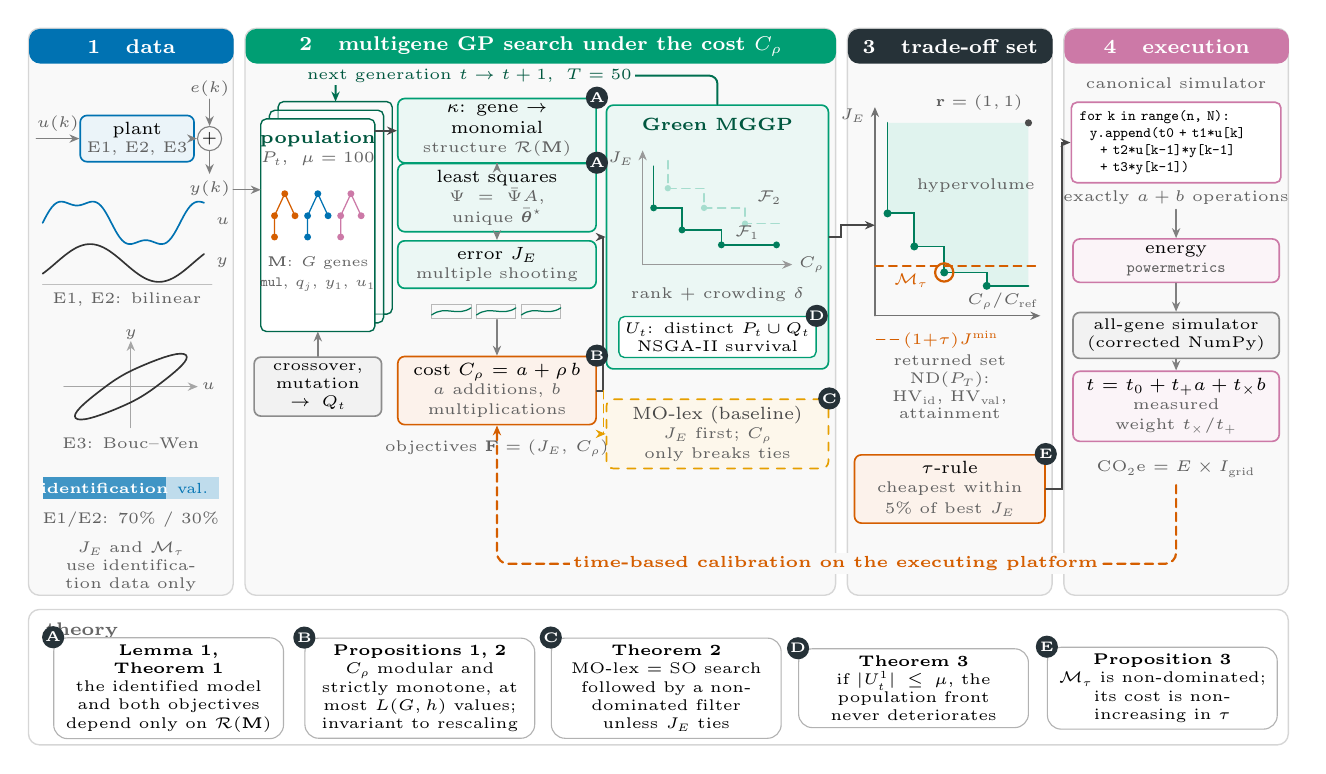
\begin{tikzpicture}[
  x=1cm, y=1cm, line cap=round,
  font=\fontsize{6.4}{7.4}\selectfont,
  >={Stealth[length=3.6pt,width=3pt]},
  stage/.style={draw=black!16, fill=black!2.5, rounded corners=4pt, line width=0.5pt},
  head/.style={rounded corners=4pt, text=white, font=\fontsize{7.2}{8}\selectfont\bfseries,
               minimum height=0.44cm, inner sep=2pt, anchor=north west},
  box/.style={draw=#1, fill=#1!8, rounded corners=2.5pt, line width=0.6pt, align=center, inner sep=2.4pt},
  box/.default=black,
  gbox/.style={draw=black!45, fill=black!5, rounded corners=2.5pt, line width=0.6pt, align=center, inner sep=2.4pt},
  lbl/.style={font=\fontsize{5.6}{6.5}\selectfont, text=black!62, align=center},
  flow/.style={->, line width=0.7pt, draw=black!72},
  thin/.style={->, line width=0.5pt, draw=black!50},
  badge/.style={draw=black!30, fill=white, rounded corners=5pt, align=center, inner sep=2.4pt,
                font=\fontsize{5.6}{6.6}\selectfont, text width=#1},
  badge/.default=2.6cm,
  tag/.style={circle, fill=cInk, text=white, font=\fontsize{5}{5}\selectfont\bfseries, inner sep=0pt,
              minimum size=8pt},
]
\definecolor{cData}{HTML}{0072B2}
\definecolor{cGreen}{HTML}{009E73}
\definecolor{cLex}{HTML}{E69F00}
\definecolor{cCost}{HTML}{D55E00}
\definecolor{cExec}{HTML}{CC79A7}
\definecolor{cInk}{HTML}{263238}
\def\sub{\fontsize{5.6}{6.5}\selectfont\color{black!62}}

% ================================================================= stage frames
\draw[stage] (0,1.9) rectangle (2.6,9.1);
\draw[stage] (2.75,1.9) rectangle (10.25,9.1);
\draw[stage] (10.4,1.9) rectangle (13.0,9.1);
\draw[stage] (13.15,1.9) rectangle (16,9.1);
\node[head, fill=cData,  minimum width=2.6cm]  at (0,9.1)     {1\quad data};
\node[head, fill=cGreen, minimum width=7.5cm]  at (2.75,9.1)  {2\quad multigene GP search under the cost $C_\rho$};
\node[head, fill=cInk,   minimum width=2.6cm]  at (10.4,9.1)  {3\quad trade-off set};
\node[head, fill=cExec,  minimum width=2.85cm] at (13.15,9.1) {4\quad execution};

% ================================================================= 1  DATA
\node[box=cData, minimum width=1.05cm, minimum height=0.5cm] (plant) at (1.38,7.7) {plant\\[-1pt]\sub E1, E2, E3};
\draw[thin] (0.1,7.7) -- node[above, lbl, pos=0.5, yshift=-1pt]{$u(k)$} (plant.west);
\node[draw=black!50, circle, inner sep=0.5pt, font=\fontsize{5.5}{5}\selectfont] (sum) at (2.3,7.7) {$+$};
\draw[thin] (plant.east) -- (sum.west);
\draw[thin] (2.3,8.2) node[above, lbl, yshift=-2.5pt]{$e(k)$} -- (sum.north);
\draw[thin] (sum.south) -- (2.3,7.25) node[below, lbl, yshift=1pt]{$y(k)$};
\begin{scope}[shift={(0.18,5.85)}]
  \draw[black!25, line width=0.35pt] (0,0) -- (2.15,0);
  \draw[cData, line width=0.6pt, domain=0:2.05, samples=70, smooth]
     plot (\x, {0.3*sin(deg(3.6*\x)) + 0.08*sin(deg(10.8*\x)) + 0.78});
  \draw[black!80, line width=0.6pt, domain=0:2.05, samples=70, smooth]
     plot (\x, {0.24*sin(deg(3.6*\x - 0.6)) + 0.27});
  \node[lbl, anchor=west] at (2.08,0.8) {$u$};
  \node[lbl, anchor=west] at (2.08,0.27) {$y$};
  \node[lbl] at (1.07,-0.2) {E1, E2: bilinear};
\end{scope}
\begin{scope}[shift={(1.3,4.55)}]
  \draw[->, black!35, line width=0.35pt] (-0.85,0) -- (0.85,0) node[right, lbl, xshift=-2pt]{$u$};
  \draw[->, black!35, line width=0.35pt] (0,-0.52) -- (0,0.58) node[above, lbl, yshift=-3pt]{$y$};
  \draw[black!80, line width=0.6pt, smooth cycle, tension=0.85]
    plot coordinates {(-0.7,-0.4) (-0.18,-0.28) (0.4,0.06) (0.7,0.4) (0.18,0.28) (-0.4,-0.06)};
  \node[lbl] at (0,-0.72) {E3: Bouc--Wen};
\end{scope}
\fill[cData!75] (0.18,3.12) rectangle (1.75,3.4);
\fill[cData!25] (1.75,3.12) rectangle (2.42,3.4);
\node[font=\fontsize{5.3}{6}\selectfont\bfseries, text=white] at (0.965,3.26) {identification};
\node[font=\fontsize{5.3}{6}\selectfont, text=cData] at (2.085,3.26) {val.};
\node[lbl, anchor=north] at (1.3,3.08) {E1/E2: $70\%$ / $30\%$};
\node[lbl, align=center, anchor=north, text width=2.35cm] at (1.3,2.7)
  {$J_E$ and $\mathcal M_\tau$ use identification data only};

% ================================================================= 2  SEARCH
\foreach \o/\op in {0.22/0.3, 0.11/0.55, 0/1} {
  \draw[draw=cGreen!65!black, fill=white, fill opacity=\op, rounded corners=2pt, line width=0.5pt]
     (2.95+\o,5.25+\o) rectangle (4.4+\o,7.95+\o);
}
\node[font=\fontsize{6.4}{7}\selectfont\bfseries, text=cGreen!55!black] at (3.675,7.7) {population};
\node[lbl] at (3.675,7.45) {$P_t$,\; $\mu=100$};
\foreach \gx/\gc in {3.255/cCost, 3.675/cData, 4.095/cExec} {
  \draw[\gc, line width=0.45pt] (\gx,7.0) -- (\gx-0.13,6.72) (\gx,7.0) -- (\gx+0.13,6.72) (\gx-0.13,6.72) -- (\gx-0.13,6.45);
  \foreach \p in {(\gx,7.0),(\gx-0.13,6.72),(\gx+0.13,6.72),(\gx-0.13,6.45)} \fill[\gc] \p circle (1.25pt);
}
\node[lbl, font=\fontsize{5.1}{6}\selectfont] at (3.675,6.12) {$\mathbf M$: $G$ genes};
\node[lbl, font=\fontsize{5.1}{6}\selectfont] at (3.675,5.85) {\texttt{mul}, $q_j$, $y_1$, $u_1$};
\node[gbox, text width=1.45cm, font=\fontsize{5.6}{6.5}\selectfont] (var) at (3.675,4.55)
  {crossover,\\ mutation $\to Q_t$};
\draw[thin] (var.north) -- (3.675,5.25);
\draw[thin] (2.6,7.05) -- (2.95,7.05);

% evaluation column
\def\ex{5.95}
\node[box=cGreen, text width=2.35cm] (kappa) at (\ex,7.8)
  {$\kappa$: gene $\to$ monomial\\[-0.5pt]\sub structure $\mathcal R(\mathbf M)$};
\node[box=cGreen, text width=2.35cm] (ls) at (\ex,6.95)
  {least squares\\[-0.5pt]\sub $\Psi=\bar\Psi A$,\; unique $\bar{\boldsymbol\theta}^\star$};
\node[box=cGreen, text width=2.35cm] (je) at (\ex,6.1)
  {error $J_E$\\[-0.5pt]\sub multiple shooting};
\begin{scope}[shift={(\ex-0.83,5.42)}]
  \foreach \w in {0,0.57,1.14} {
    \draw[black!28, line width=0.35pt] (\w,0) rectangle (\w+0.5,0.17);
    \draw[cGreen!75!black, line width=0.45pt] (\w,0.04) .. controls (\w+0.18,0.17) and (\w+0.32,0.01) .. (\w+0.5,0.13);
  }
\end{scope}
\node[box=cCost, text width=2.35cm] (cost) at (\ex,4.5)
  {cost $C_\rho=a+\rho\,b$\\[-0.5pt]\sub $a$ additions, $b$ multiplications};
\draw[flow] (4.4,7.8) -- (kappa.west);
\draw[thin] (kappa) -- (ls);
\draw[thin] (ls) -- (je);
\draw[thin] (\ex,5.4) -- (cost.north);
\node[lbl, anchor=north] at (\ex,4.0) {objectives $\mathbf F=(J_E,\,C_\rho)$};

% selection column
\def\sx{8.75}
\node[box=cGreen, text width=2.65cm, minimum height=3.35cm] (green) at (\sx,6.45) {};
\node[font=\fontsize{6.4}{7}\selectfont\bfseries, text=cGreen!55!black] at (\sx,7.88) {Green MGGP};
\begin{scope}[shift={(\sx-0.95,6.1)}]
  \draw[->, black!40, line width=0.35pt] (0,0) -- (1.9,0) node[right, lbl, xshift=-1pt]{$C_\rho$};
  \draw[->, black!40, line width=0.35pt] (0,0) -- (0,1.45) node[left, lbl, yshift=-3pt]{$J_E$};
  \draw[cGreen!35, line width=0.5pt, densely dashed] (0.32,1.32) -- (0.32,0.97) -- (0.78,0.97) -- (0.78,0.72) -- (1.3,0.72) -- (1.3,0.52) -- (1.75,0.52);
  \draw[cGreen!80!black, line width=0.55pt] (0.14,1.25) -- (0.14,0.72) -- (0.5,0.72) -- (0.5,0.44) -- (1.0,0.44) -- (1.0,0.25) -- (1.7,0.25);
  \foreach \p in {(0.32,0.97),(0.78,0.72),(1.3,0.52)} \fill[cGreen!35] \p circle (1.15pt);
  \foreach \p in {(0.14,0.72),(0.5,0.44),(1.0,0.25),(1.7,0.25)} \fill[cGreen!80!black] \p circle (1.25pt);
  \node[lbl, anchor=west] at (1.05,0.4) {$\mathcal F_1$};
  \node[lbl, anchor=west] at (1.33,0.85) {$\mathcal F_2$};
\end{scope}
\node[lbl] at (\sx,5.72) {rank $+$ crowding $\delta$};
\node[draw=cGreen, fill=white, rounded corners=2pt, line width=0.5pt, text width=2.35cm, align=center,
      inner sep=2.2pt, font=\fontsize{5.6}{6.5}\selectfont] (surv) at (\sx,5.18)
  {$U_t$: distinct $P_t\cup Q_t$\\ NSGA-II survival};
\node[box=cLex, text width=2.65cm, dashed, text=black!72] (lex) at (\sx,3.95)
  {MO-lex (baseline)\\[-0.5pt]\sub $J_E$ first; $C_\rho$ only breaks ties};
\draw[flow] (cost.east) -- (7.3,4.5) |- (green.west);
\draw[thin, cLex, densely dashed] (7.3,4.5) |- (lex.west);
% generation loop above the evaluation column
\draw[flow, cGreen!70!black, rounded corners=3pt] (green.north) -- (\sx,8.5) -- (3.9,8.5) -- (3.9,8.17);
\node[font=\fontsize{5.6}{6.5}\selectfont, text=cGreen!55!black, fill=black!2.5, inner sep=1pt] at (5.6,8.5)
  {next generation $t\to t+1$,\; $T=50$};

% ================================================================= 3  TRADE-OFF SET
\begin{scope}[shift={(10.75,5.45)}]
  \fill[cGreen!12] (0.16,2.45) -- (0.16,1.3) -- (0.5,1.3) -- (0.5,0.88) -- (0.88,0.88) -- (0.88,0.55) -- (1.42,0.55) -- (1.42,0.38) -- (1.95,0.38) -- (1.95,2.45) -- cycle;
  \draw[->, black!55, line width=0.45pt] (0,0) -- (2.1,0);
  \node[lbl, anchor=south east, inner sep=1pt] at (2.12,0.04) {$C_\rho/C_\mathrm{ref}$};
  \draw[->, black!55, line width=0.45pt] (0,0) -- (0,2.65) node[left, lbl, yshift=-3pt]{$J_E$};
  \draw[cGreen!80!black, line width=0.65pt] (0.16,2.45) -- (0.16,1.3) -- (0.5,1.3) -- (0.5,0.88) -- (0.88,0.88) -- (0.88,0.55) -- (1.42,0.55) -- (1.42,0.38) -- (1.95,0.38);
  \foreach \p in {(0.16,1.3),(0.5,0.88),(0.88,0.55),(1.42,0.38)} \fill[cGreen!80!black] \p circle (1.45pt);
  \fill[black!70] (1.95,2.45) circle (1.3pt);
  \node[lbl, anchor=south east] at (2.0,2.48) {$\mathbf r=(1,1)$};
  \node[lbl] at (1.28,1.65) {hypervolume};
  \draw[cCost, densely dashed, line width=0.5pt] (0,0.63) -- (2.05,0.63);
  \draw[cCost, densely dashed, line width=0.5pt] (0.02,-0.3) -- (0.3,-0.3);
  \node[lbl, text=cCost, anchor=west, inner sep=1pt] at (0.32,-0.3) {$(1{+}\tau)J^{\min}$};
  \draw[cCost, line width=0.8pt] (0.88,0.55) circle (3.3pt);
  \node[lbl, text=cCost, anchor=east] at (0.8,0.45) {$\mathcal M_\tau$};
\end{scope}
\draw[flow] (green.east) -- ++(0.15,0) |- (10.75,6.6);
\node[lbl, text width=2.45cm] at (11.7,4.55) {returned set $\ND(P_T)$:\\ $\HV_\mathrm{id}$, $\HV_\mathrm{val}$, attainment};
\node[box=cCost, text width=2.25cm] (taurule) at (11.7,3.25)
  {$\tau$-rule\\[-0.5pt]\sub cheapest within $5\%$ of best $J_E$};

% ================================================================= 4  EXECUTION
\def\qx{14.575}
\node[lbl] at (\qx,8.4) {canonical simulator};
\node[draw=cExec, fill=white, rounded corners=2pt, line width=0.6pt, inner sep=3pt, align=left,
      font=\fontsize{5.2}{6.1}\selectfont\ttfamily, text width=2.45cm] (code) at (\qx,7.65)
  {for k in range(n, N):\\
   \ \ y.append(t0 + t1*u[k]\\
   \ \ \ \ + t2*u[k-1]*y[k-1]\\
   \ \ \ \ + t3*y[k-1])};
\node[lbl] at (\qx,6.95) {exactly $a+b$ operations};
\draw[flow] (taurule.east) -- ++(0.2,0) |- (code.west);
\node[box=cExec, text width=2.45cm] (meter) at (\qx,6.15)
  {energy\\[-0.5pt]\sub \texttt{powermetrics}};
\node[gbox, text width=2.45cm, font=\fontsize{5.6}{6.5}\selectfont] (pkg) at (\qx,5.2)
  {all-gene simulator\\ (corrected NumPy)};
\node[box=cExec, text width=2.45cm] (calib) at (\qx,4.3)
  {$t=t_0+t_+a+t_\times b$\\[-0.5pt]\sub measured weight $t_\times/t_+$};
\node[lbl] at (\qx,3.5) {CO$_2$e $=E\times I_\mathrm{grid}$};
\draw[thin] (\qx,6.8) -- (meter.north);
\draw[thin] (meter) -- (pkg);
\draw[thin] (pkg) -- (calib);
\draw[->, line width=0.8pt, cCost, densely dashed, rounded corners=4pt]
  (\qx,3.3) -- (\qx,2.3) -- (\ex,2.3) -- (cost.south);
\node[font=\fontsize{5.8}{6.6}\selectfont\bfseries, text=cCost, fill=black!2.5, inner sep=1.2pt] at (10.25,2.3)
  {time-based calibration on the executing platform};

% ================================================================= theory band
\draw[stage, fill=white] (0,0) rectangle (16,1.72);
\node[font=\fontsize{6.6}{7.6}\selectfont\bfseries, text=black!60, anchor=north west] at (0.1,1.68) {theory};
\node[badge=2.75cm] (b1) at (1.78,0.72)  {\textbf{Lemma 1, Theorem 1}\\ the identified model and both objectives depend only on $\mathcal R(\mathbf M)$};
\node[badge=2.75cm] (b2) at (4.97,0.72)  {\textbf{Propositions 1, 2}\\ $C_\rho$ modular and strictly monotone, at most $L(G,h)$ values; invariant to rescaling};
\node[badge=2.75cm] (b3) at (8.1,0.72)   {\textbf{Theorem 2}\\ MO-lex $=$ SO search followed by a non-dominated filter unless $J_E$ ties};
\node[badge=2.75cm] (b4) at (11.24,0.72) {\textbf{Theorem 3}\\ if $|U_t^1|\le\mu$, the population front never deteriorates};
\node[badge=2.75cm] (b5) at (14.4,0.72)  {\textbf{Proposition 3}\\ $\mathcal M_\tau$ is non-dominated; its cost is non-increasing in $\tau$};
\foreach \b/\t in {b1/A, b2/B, b3/C, b4/D, b5/E} \node[tag] at (\b.north west) {\t};
\node[tag] at (kappa.north east) {A};
\node[tag] at (ls.north east) {A};
\node[tag] at (cost.north east) {B};
\node[tag] at (lex.north east) {C};
\node[tag] at (surv.north east) {D};
\node[tag] at (taurule.north east) {E};
\end{tikzpicture}
}
\caption{Overview of the identification and execution workflow. Data feed a common estimator and predictor; Green uses Pareto ranking and crowding, while MO-lex compares fitness lexicographically. The identification-only $\tau$-rule selects one model from the delivered set. Timing assesses the fixed weights; powermetrics measures energy and CodeCarbon supplies grid carbon intensity. The dashed path denotes calibration for a subsequent search, not retrospective retuning. Letters A--E identify the structural, cost and selection properties explained in the methodology. Timing and energy are separate measurements within stage 4; the arrows indicate the execution-stage workflow. The 70\%/30\% split applies to E1/E2; E3 uses separate records.}
\label{fig:pipeline}
\end{figure}

\subsection{Representation and the executed polynomial}
An individual is a collection $\M=(g_1,\ldots,g_G)$ of gene trees. The grammar uses terminals $y_1=y(k-1)$ and $u_1=u(k)$, multiplication and a delay $q_j$ of the whole subtree. Thus every gene denotes a monomial of delayed signals~\cite{Searson2015,mggpy}. For example, $q_1(\mathrm{mul}(y_1,u_1))$ denotes $y(k-2)u(k-1)$: the operator shifts both factors. For a monomial $m$, let $m_{v,\ell}$ denote the exponent of signal $v\in\{y,u\}$ at delay $\ell$. Its regressor and degree are
\begin{equation}
\varphi_m(k)=\prod_{v\in\{y,u\}}\prod_{\ell\ge0}v(k-\ell)^{m_{v,\ell}},
\qquad d_m=\sum_{v,\ell}m_{v,\ell}.
\label{eq:monomial}
\end{equation}
Only finitely many exponents are non-zero, and output factors have positive delays. Let $\kappa(g_i)$ be the monomial denoted by gene $g_i$. The executed structure is the set
\begin{equation}
\mathcal R(\M)=\{\kappa(g_i):i=1,\ldots,G\},\qquad
n=\max\{\ell:m_{v,\ell}>0,\ m\in\mathcal R(\M)\}.
\label{eq:structure}
\end{equation}
Taking a set removes repeated monomials, regardless of differences in tree syntax. The actual maximum factor delay $n$ determines the required history. With one intercept and one coefficient per distinct regressor, the executed model is
\begin{equation}
\hat y(k)=\theta_0+\sum_{m\in\mathcal R(\M)}\bar\theta_m\varphi_m(k).
\label{eq:model}
\end{equation}
Figure~\ref{fig:schematic} illustrates how the representation can contain more genes than the executed polynomial contains regressors.

\subsection{Least-squares estimation and duplicate aggregation}
Estimation uses identification data only. With sample indices $k=0,\ldots,N_{\mathrm{id}}-1$, the regression matrix has rows
\begin{equation}
\Psi_{k,:}=[1,\ \varphi_{\kappa(g_1)}(k),\ldots,\varphi_{\kappa(g_G)}(k)],
\qquad k=n,\ldots,N_{\mathrm{id}}-1.
\end{equation}
All factors in this matrix use measured inputs and outputs. The estimator retains one column per gene, including repeated columns, and solves
\begin{equation}
\hat{\boldsymbol\theta}\in\arg\min_{\boldsymbol\theta}
\|\mathbf y-\Psi\boldsymbol\theta\|_2^2,
\qquad
\bar\theta_m=\sum_{i:\kappa(g_i)=m}\hat\theta_i.
\label{eq:ls}
\end{equation}
The intercept is retained separately. Aggregating duplicate coefficients leaves the polynomial unchanged. If the matrix with one column per distinct monomial has full column rank, its fitted canonical coefficients are unique even when the gene-level coefficients are not. This is the structural-invariance property marked A in Fig.~\ref{fig:pipeline}.

A shared external evaluator implements the intended delays in both estimation and simulation. It allocates history from $n$ in \eqref{eq:structure}, avoids circular-buffer indexing and does not replace divergent predictions by zeros. Input-only models and delayed mixed products follow the same factor semantics. These corrections apply equally to all compared methods; the vendored MGGP package and the genetic operators remain unchanged.

\begin{figure}[!htbp]\centering
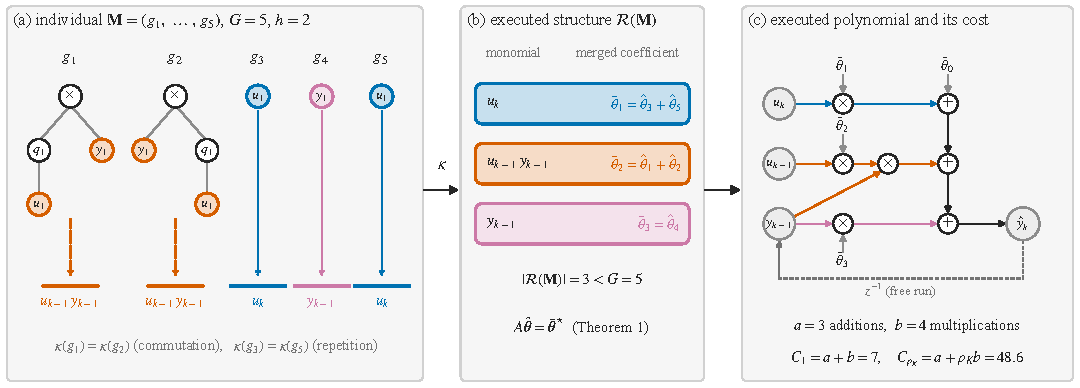
\includegraphics[width=\textwidth]{figures/fig_schematic.pdf}
\caption{Mapping gene trees to the executed polynomial and its arithmetic cost. Five gene trees collapse into three distinct monomials; coefficients of duplicate genes are merged. Direct execution counts additions and multiplications, including coefficient multiplications. This illustrative E1 model omits the true bilinear regressor and is not the generating structure.}
\label{fig:schematic}
\end{figure}

\subsection{Recursive prediction and error objectives}
Once coefficients are estimated, each model is simulated recursively. In a validation record, define $\widetilde y(k)=y(k)$ for $0\le k<n$ and $\widetilde y(k)=\hat y(k)$ thereafter. The free-run predictor is
\begin{equation}
\hat y(k)=\theta_0+\sum_{m\in\mathcal R}\bar\theta_m
\prod_{\ell\ge1}\widetilde y(k-\ell)^{m_{y,\ell}}
\prod_{\ell\ge0}u(k-\ell)^{m_{u,\ell}},\qquad k\ge n.
\label{eq:freerun}
\end{equation}
After initialisation, output regressors therefore use predictions rather than measured outputs. Inputs remain the supplied excitation. For input-only structures with $n=0$, no output history is needed.

Identification uses multiple shooting with horizon $K=20$. The identification record is divided into $W=\lfloor N_{\mathrm{id}}/(n+K)\rfloor$ complete, non-overlapping windows. Each window starts with $n$ measured outputs and then applies \eqref{eq:freerun} for $K$ steps. Remaining samples outside complete windows are not included. If $y_w(j)$ and $\hat y_w(j)$ are measured and simulated outputs within window $w$, the reported objective is
\begin{equation}
J_E=\frac{1}{\sigma_{\mathrm{id}}}
\sqrt{\frac{1}{W(n+K)}\sum_{w=1}^{W}\sum_{j=0}^{n+K-1}
\big(y_w(j)-\hat y_w(j)\big)^2}.
\label{eq:je}
\end{equation}
Here $\sigma_{\mathrm{id}}$ is the standard deviation of the identification output. The first $n$ residuals in each window are zero and remain in the normalisation. The search uses the unnormalised RMSE; division by a fixed $\sigma_{\mathrm{id}}$ does not change its ordering. This reset-window criterion has no optimised initial states or continuity constraints~\cite{Ribeiro2020}. Failed estimation or a non-finite simulation is recorded as infinite error.

Validation is a separate uninterrupted free run, without refitting on validation data or resetting intermediate outputs. Its NRMSE excludes the initial history:
\begin{equation}
J_{\mathrm{val}}=\frac{1}{\sigma_{\mathrm{val},n}}
\sqrt{\frac{1}{N_{\mathrm{val}}-n}\sum_{k=n}^{N_{\mathrm{val}}-1}
\big(y(k)-\hat y(k)\big)^2},
\label{eq:validation}
\end{equation}
where $\sigma_{\mathrm{val},n}$ is the standard deviation of the measured validation outputs on those same scored samples. Validation is used to assess the delivered models, not to direct search or choose the final model.

\subsection{Arithmetic complexity and the two declared weights}
Complexity is computed from the duplicate-free polynomial, not measured from its runtime. A monomial of degree $d_m$ requires $d_m-1$ factor multiplications and one coefficient multiplication. Adding it to the running sum requires one addition. Thus
\begin{equation}
a=|\mathcal R|,\qquad b=\sum_{m\in\mathcal R}d_m,\qquad
C_\rho=\sum_{m\in\mathcal R}(1+\rho d_m)=a+\rho b.
\label{eq:cost}
\end{equation}
The intercept does not add a separate multiplication. All structural regressors are counted, including those with small fitted coefficients; no coefficient threshold removes terms. A duplicated gene adds no new canonical operations. Units are addition-equivalents, and $C_\rho$ is an operation model rather than measured energy.

Both weights were fixed before the searches. The primary $\rho=1$ gives $C_1=a+b$. The secondary uses the Green-Box bit-level model~\cite{NMN2023}, where addition costs $B$ and Karatsuba multiplication costs $B^\alpha$, $\alpha=\log_2 3$~\cite{KO1963}:
\begin{equation}
\rho_K=B^{\alpha-1}=\frac{729}{64}\quad(B=64),\qquad
B C_{\rho_K}=Ba+B^\alpha b.
\label{eq:karatsuba}
\end{equation}
This theoretical weight does not measure binary64 instruction costs on this laptop. Timing later checks an implementation-specific multiplication-to-addition ratio; neither power measurements nor CodeCarbon establishes $\rho$.

Adding a distinct regressor strictly increases $C_\rho$, and costs add over sets of regressors (property B). A strictly increasing transformation of the entire cost preserves Pareto and lexicographic ordering, but changing $\rho$ changes the relative weights of $a$ and $b$ and can reverse structure orderings. No weight is tuned to favour search outcomes.

\subsection{Pareto selection, lexicographic selection and the generation cycle}
The Green objective vector is $\F(\M)=(J_E(\M),C_\rho(\M))$. Model $\M$ dominates $\M'$ when
\begin{equation}
J_E(\M)\le J_E(\M'),\quad C_\rho(\M)\le C_\rho(\M'),
\quad\text{with at least one strict inequality}.
\label{eq:dominance}
\end{equation}
Non-dominated sorting assigns rank 1 to models dominated by none, then successive ranks after removing earlier fronts. Within each front, NSGA-II crowding distance favours less densely represented regions~\cite{DPAM2002}. For an interior individual,
\begin{equation}
\delta(\M)=\sum_{q=1}^{2}
\frac{F_q(\M_q^+)-F_q(\M_q^-)}{F_q^{\max}-F_q^{\min}},
\label{eq:crowding}
\end{equation}
where neighbours are sorted by objective $q$ within that front. Boundary individuals receive infinite distance; constant-objective contributions are skipped. A crowded binary tournament prefers lower rank and, on a rank tie, higher crowding distance.

SO instead compares error alone and returns its Hall-of-Fame model. MO-lex supplies both objectives but the package's DEAP fitness comparison is lexicographic~\cite{FDG+2012,DEAPFitness}:
\begin{equation}
\M<_{\mathrm{lex}}\M'\iff
J_E(\M)<J_E(\M')\ \text{or}\
\big[J_E(\M)=J_E(\M')\ \text{and}\ C_\rho(\M)<C_\rho(\M')\big].
\end{equation}
Cost therefore changes its decisions only on error ties. With the same initial population and random stream, SO and MO-lex follow identical trajectories whenever equal-error comparisons also have equal costs (property C). Their delivered outputs still differ: SO gives one model, whereas MO-lex extracts the final non-dominated set.

\begin{algorithm}[!htbp]
\caption{Green MGGP with the common equal-evaluation protocol}
\label{alg:sharing}
\begin{algorithmic}[1]
\Require identification data; fixed $\rho$; $\mu=100$; $\lambda=90$; 49 evolutionary steps
\State initialise 100 individuals; estimate coefficients and evaluate every individual
\For{each evolutionary step}
\State rank the current population and assign crowding distances
\State select $\lambda$ parents by crowded binary tournament and copy them
\State apply the shared crossover and mutation operators to the copies
\State estimate coefficients and evaluate all $\lambda$ offspring, including unchanged copies
\State form the parent--offspring union and remove structural duplicates among finite candidates
\State retain $\mu$ individuals by Pareto rank and crowding; fill remaining places if needed
\EndFor
\State deliver the distinct non-dominated final models; apply the identification-only $\tau$-rule
\State evaluate the same delivered models in uninterrupted validation free run
\end{algorithmic}
\end{algorithm}
The algorithm preserves search variation settings and changes parent and survivor selection. For the term/node ablations, the second objective is replaced by the declared complexity measure; arithmetic cost still assesses their delivered sets. If the first front of the de-duplicated union fits in the population, Green retains it and its population-front hypervolume cannot decrease (property D). This is a conditional statement, not a guarantee for arbitrary front sizes.

\subsection{Choosing one model and assessing delivered sets}
Let $\mathcal P$ be a delivered set and $J_E^{\min}=\min_{\M\in\mathcal P}J_E(\M)$. The fixed selection rule is
\begin{equation}
\mathcal M_\tau\in\arg\min_{\M\in\mathcal P}\left\{C_\rho(\M):
J_E(\M)\le(1+\tau)J_E^{\min}+\eta\right\},
\quad\tau=0.05,\quad\eta=10^{-6}.
\label{eq:tau}
\end{equation}
It chooses the cheapest delivered model within the declared identification-error tolerance (property E); for SO, the singleton is already the selected model. Validation does not enter this choice. A model with better validation elsewhere in the set is a diagnostic, not a replacement selected after observing outcomes.

Hypervolume measures a delivered set in normalised cost--error coordinates~\cite{ZT1999}. For $G$ genes and maximum tree height $h$, each monomial degree is at most $D=2^h$, so the declared bound is
\begin{equation}
C_{\mathrm{ref}}=G(1+\rho 2^h),\qquad
\HV(\mathcal P)=\operatorname{area}\!\left(
\bigcup_{\M\in\mathcal P}
[C_\rho(\M)/C_{\mathrm{ref}},1]\times[J(\M),1]\right).
\label{eq:hv}
\end{equation}
Only points within the reference $(1,1)$ contribute. Set $J=J_E$ for identification HV and $J=J_{\mathrm{val}}$ for validation HV of the same models. Higher values indicate a larger dominated region. SO's singleton and the multi-model outputs differ in format, so this comparison alone does not isolate search quality. Changing $\rho$ also changes the cost coordinate; HV values under different weights are not interchangeable.

\section{Experimental comparison}
E1 is the noise-free tutorial system
\begin{equation}
y(k)=0.65y(k-1)+0.35u(k)+0.10u(k)y(k-1),\label{eq:tutorial}
\end{equation}
with input $u=\sin t+0.25\sin3t$ and 300 samples split 70\%/30\%. E2 adds Gaussian output noise with standard deviation 0.02 and fixed noise seed 2027. E3 is the package's Bouc--Wen system~\cite{IR2007}, with separate identification and validation excitations. Its equations are
\begin{equation}
y=d_pu-h,\qquad
\dot h=A\dot u-\beta|\dot u|h-\gamma\dot u|h|.
\label{eq:boucwen}
\end{equation}
The parameters are $A=0.9$, $\beta=\gamma=0.008$, $d_p=1.6$, integrated by RK4 at 1~ms and decimated by 20. Identification uses a 1~Hz sine of amplitude 20--50 over 6~s; validation uses a 0.8~Hz sine of amplitude 45 over 4~s.
\begin{table}[!htbp]
\centering
\caption{Examples and search settings; $C_\mathrm{ref}$ for $\rho=1$ (common: population 100, 50 generations, crossover 0.9, initial mutation 0.2; baseline elite retention 10\%, multiple-shooting horizon $K=20$, primitives \texttt{mul} and $q^{-j}$).}
\label{tab:setup}
\setlength{\tabcolsep}{4pt}
\begin{tabular}{lcccccc}
\toprule
Example & $N_\mathrm{id}$ & $N_\mathrm{val}$ & genes & height & $j_{\max}$ & $C_\mathrm{ref}$ \\
\midrule
E1 Tutorial (noise-free) & 210 & 90 & 5 & 2 & 2 & 25 \\
E2 Tutorial (noisy) & 210 & 90 & 5 & 2 & 2 & 25 \\
E3 Bouc--Wen hysteresis & 300 & 200 & 8 & 3 & 3 & 72 \\
\bottomrule
\end{tabular}
\end{table}


The principal comparison evaluates 100 initial individuals and 90 offspring at each of 49 steps, including unchanged offspring and failures: exactly 4,510 fitness calls per run. Fifty recorded generations include the initial population. Mutation starts at 0.2 and increases by 0.1, up to 0.9, at nine-generation checkpoints when improvement is below 5\%. In addition to SO, MO-lex and Green, two Pareto ablations minimise distinct terms or all representation nodes; node de-duplication retains the smallest representation. Each configuration uses 30 independent seeds per example under both weights. The 900 equal-evaluation runs and 540 native-budget diagnostic runs give 1,440 runs in total.

The objectives, final selection rule and set indicators are defined in \eqref{eq:je}--\eqref{eq:hv}. Failed runs or simulations remain infinite or missing, with counts retained alongside finite-error medians. Comparisons use two-sided Mann--Whitney tests, Holm correction and Vargha--Delaney $A_{12}$~\cite{MW1947,Hol1979,VD2000}; runs are not paired. The equal-evaluation analysis corrects 60 tests per weight, including the ablations. Reference-point sensitivity is a separate analysis, not a new choice of the primary indicator.

\section{Corrected results and interpretation}
\begin{table*}[!htbp]
\centering
\caption{Results over 30 independent runs with $\rho=1$: median [interquartile range]. HV: hypervolume of the delivered set (identification or free-run validation error); $C_\tau$, NRMSE$_\tau$: cost and free-run validation NRMSE of the model selected by the $\tau$-rule; Rec.$_\tau$, Rec.$_\mathcal{P}$: fraction of runs in which the selected model, or at least one model of the returned set, contains the three true regressors of \eqref{eq:tutorial}. $^{\ast}$/$^{\dagger}$: Green differs from SO/MO-lex (Mann--Whitney, Holm-adjusted $p<0.05$).}
\label{tab:results}
\footnotesize
\setlength{\tabcolsep}{2.5pt}
\resizebox{\textwidth}{!}{%
\begin{tabular}{llcccccc}
\toprule
Ex. & Method & HV$_\mathrm{id}$ & HV$_\mathrm{val}$ & $C_\tau$ & NRMSE$_\tau$ & Rec.$_\tau$ & Rec.$_\mathcal{P}$ \\
\midrule
\multirow{3}{*}{E1} & SO & 0.640 [0.560, 0.640] & 0.640 [0.560, 0.640] & 9 [9, 11] & 3e-16 [2e-16, 3e-16] & 1.00 & 1.00 \\
 & MO-lex & 0.829 [0.803, 0.829] & 0.827 [0.798, 0.827] & 7 [7, 7] & 3e-16 [3e-16, 3e-16] & 1.00 & 1.00 \\
 & \textbf{Green} & 0.896 [0.896, 0.896]$^{\ast}$$^{\dagger}$ & 0.893 [0.893, 0.893]$^{\ast}$$^{\dagger}$ & 7 [7, 7]$^{\ast}$ & 9e-16 [7e-16, 2e-15]$^{\ast}$$^{\dagger}$ & 1.00 & 1.00 \\
\midrule
\multirow{3}{*}{E2} & SO & 0.508 [0.508, 0.508] & 0.505 [0.505, 0.505] & 12 [12, 12] & 0.028 [0.028, 0.028] & 0.00 & 0.00 \\
 & MO-lex & 0.702 [0.661, 0.703] & 0.699 [0.656, 0.700] & 10 [9, 10] & 0.028 [0.028, 0.029] & 0.00 & 0.07 \\
 & \textbf{Green} & 0.878 [0.878, 0.879]$^{\ast}$$^{\dagger}$ & 0.872 [0.872, 0.874]$^{\ast}$$^{\dagger}$ & 7 [7, 7]$^{\ast}$$^{\dagger}$ & 0.028 [0.028, 0.028] & 0.00 & 0.00 \\
\midrule
\multirow{3}{*}{E3} & SO & 0.736 [0.729, 0.770] & 0.000 [0.000, 0.000] & 18.5 [16, 19] & 1.394 [1.301, 1.463] & -- & -- \\
 & MO-lex & 0.798 [0.797, 0.825] & 0.000 [0.000, 0.471] & 16 [16, 16] & 1.411 [1.340, 1.467] & -- & -- \\
 & \textbf{Green} & 0.955 [0.932, 0.956]$^{\ast}$$^{\dagger}$ & 0.893 [0.868, 0.893]$^{\ast}$$^{\dagger}$ & 16 [14.5, 16]$^{\ast}$ & 1.420 [1.316, 1.451] & -- & -- \\
\bottomrule
\end{tabular}}
\end{table*}

Green's median identification HV is \EBGreenHVid, \ECGreenHVid{} and \EDGreenHVid{} on E1--E3; its validation HV is \EBGreenHVval, \ECGreenHVval{} and \EDGreenHVval. These delivered-set indicators exceed the baseline medians, but do not establish better validation for every selected model. Selected Green costs are \EBGreenCsel, \ECGreenCsel{} and \EDGreenCsel{} operations, compared with \EBSOCsel, \ECSOCsel{} and \EDSOCsel{} for SO. Cost reductions refer to differences between method medians, not paired per-run reductions.

On E1 all selected models are effectively exact; statistical distinctions below $10^{-14}$ have no practical accuracy meaning. On E2 the cheaper selected models retain similar validation NRMSE but do not recover the generating regressors; the delivered Green sets do not contain all three generating regressors in these corrected runs. E3 is more problematic: the selected Green validation NRMSE is \EDGreenVALsel, against \EDSOVALsel{} for SO and \EDLexVALsel{} for MO-lex. The Green sets contain substantially better validation models, but the identification-only rule does not choose them. The rule remains fixed rather than being retuned after validation.

\begin{figure}[!htbp]\centering
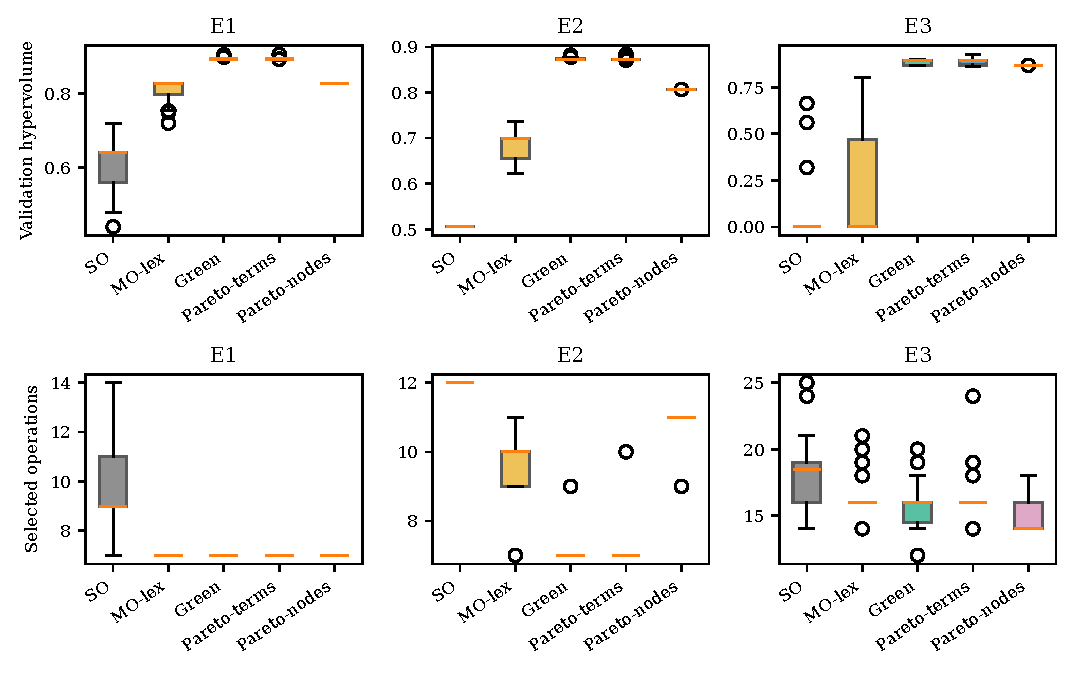
\includegraphics[width=\textwidth]{figures/fig_corrected_ablation.pdf}
\caption{Equal-evaluation ablations: validation hypervolume of the delivered sets and arithmetic cost of the selected models over 30 runs. Higher HV and lower cost are favourable, but selected-model validation must be assessed separately.}
\label{fig:ablation}
\end{figure}
Figure~\ref{fig:ablation} shows that the term-count objective has no significant difference in validation HV from Green on any example after Holm correction. The arithmetic objective describes operations explicitly, but these experiments do not establish a consistent advantage over counting terms. On E3, finite-error medians also require attention to failures: six term-ablation runs, one SO run and one MO-lex run fail validation under $\rho=1$.

\begin{table}[!htbp]
\centering
\caption{Effect of the multiplication weight $\rho$ over 30 runs (medians). HV: identification hypervolume; $\Delta C_\tau$: reduction of the median selected cost of Green MGGP relative to SO, with the cost of the same scenario; $a{+}b$ and $C_{\rho_K}$: operation count and Karatsuba-weighted cost of the selected Green model; same: fraction of seeds in which Green MGGP selects the same structure under both weights.}
\label{tab:rho}
\setlength{\tabcolsep}{3.5pt}
\small
\begin{tabular}{llccccccc}
\toprule
 & & \multicolumn{3}{c}{HV$_\mathrm{id}$} & & \multicolumn{2}{c}{Green $\mathcal M_\tau$} & \\
\cmidrule(lr){3-5}\cmidrule(lr){7-8}
Ex. & weight & SO & MO-lex & Green & $\Delta C_\tau$ & $a{+}b$ & $C_{\rho_K}$ & same \\
\midrule
E1 & $\rho=1$ & 0.640 & 0.829 & 0.896 & 22\% & 7 & 48.6 & 100\% \\
 & $\rho_K$ & 0.738 & 0.884 & 0.929 & 20\% & 7 & 48.6 &  \\
\midrule
E2 & $\rho=1$ & 0.508 & 0.702 & 0.878 & 42\% & 7 & 48.6 & 80\% \\
 & $\rho_K$ & 0.622 & 0.773 & 0.910 & 43\% & 7 & 48.6 &  \\
\midrule
E3 & $\rho=1$ & 0.736 & 0.798 & 0.955 & 14\% & 16 & 109.5 & 0\% \\
 & $\rho_K$ & 0.819 & 0.874 & 0.969 & 14\% & 16 & 109.5 &  \\
\bottomrule
\end{tabular}
\end{table}

Table~\ref{tab:rho} retains both weights and shows that selected structures can change even when their median operation counts coincide. Different weights also give different HV coordinates, so their HV values are not directly interchangeable. Population hashes confirm identical SO/MO-lex trajectories on all primary-weight runs; Green has no population-front HV drops and satisfies the observed union-front capacity condition. These empirical checks support the conditional theoretical statements, not a universal guarantee.

\section{Measured time, energy and carbon}
The new mains-powered Apple M2 session rebuilds the selected records of five groups: SO, MO-lex and Green under $\rho=1$, plus MO-lex and Green under $\rho_K$. Of 450 records, 446 pass reconstruction checks; four failed validations remain missing. The canonical simulator executes each distinct monomial once. The secondary NumPy simulator executes all genes with corrected delays. Their predictions agree within the declared tolerances.

Each timing batch lasts at least 50~ms. For \CorrectedNStructures{} distinct canonical structures, the fitted ratio is $t_\times/t_+=\CorrectedMulAdd$. The operation-count fit gives $R^2=\CorrectedRtwoOne$, compared with \CorrectedRtwoK{} for the Karatsuba-weighted cost. This supports an order-one weight in this Python implementation, including interpreter overhead; it does not retrospectively change the search weights.

Execution timing is model-specific and normalised by the number $N_s$ of predicted samples. For five batches with $r_j$ repeated simulations and elapsed time $T_j$,
\begin{equation}
t_{\mathrm{sample}}=\frac{1}{N_s}\operatorname{median}_{j=1,\ldots,5}\frac{T_j}{r_j},
\qquad t=t_0+t_+a+t_\times b,\qquad\rho_{\mathrm{time}}=t_\times/t_+.
\label{eq:timing}
\end{equation}
The regression uses distinct canonical structures and is an assessment of their Python execution, rather than an independent instruction-level benchmark.

Powermetrics samples CPU, GPU and neural-engine power every 100~ms. Ten rounds visit 30 groups in seeded random order, repeating complete cycles of each group's models for at least 10~s. Eleven idle blocks bracket the rounds: 311 valid blocks in total. Net energy is integrated block energy minus the median idle power times block duration, divided by completed simulations. For block power samples $P_i$ spanning intervals $\Delta t_i$, block duration $T_{\mathrm{block}}$ and $n_{\mathrm{sim}}$ completed simulations, the calculation is
\begin{equation}
E_{\mathrm{block}}=\sum_i P_i\Delta t_i,\qquad
E_{\mathrm{sim}}=\frac{E_{\mathrm{block}}-\widetilde P_{\mathrm{idle}}T_{\mathrm{block}}}{n_{\mathrm{sim}}}.
\label{eq:energy}
\end{equation}
Here $\widetilde P_{\mathrm{idle}}$ is the median of the idle-block mean powers. The bracketing-idle alternative leaves Holm-significance decisions unchanged. CodeCarbon provides only the Irish grid intensity, \CorrectedCI{}~gCO$_2$e/kWh~\cite{codecarbon}; carbon is energy in kWh multiplied by that intensity. With $E_{\mathrm{sim}}$ in joules, the carbon estimate in grams and the per-round energy ratio are
\begin{equation}
\mathrm{CO_2e}_{\mathrm{sim}}=\frac{E_{\mathrm{sim}}}{3.6\times10^6}I_{\mathrm{grid}},\qquad
R_r=\frac{E_{\mathrm{sim},r}^{\mathrm{Green}}}{E_{\mathrm{sim},r}^{\mathrm{SO}}}.
\label{eq:carbon}
\end{equation}
Reported energy ratios are medians of $R_r$ over rounds, distinct from reductions between search-method cost medians. Energy comparisons correct 18 tests across examples, simulators and comparators. These rounds belong to one measurement session, not independent hardware sessions.

\begin{figure}[!htbp]\centering
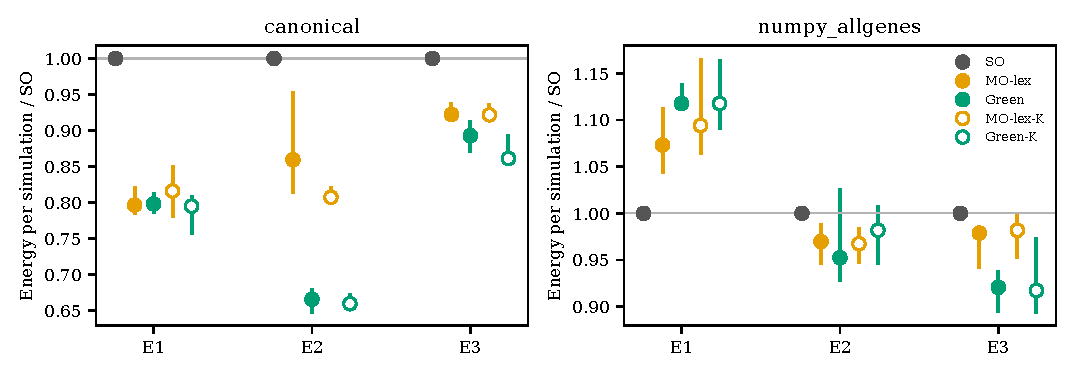
\includegraphics[width=\textwidth]{figures/fig_energy.pdf}
\caption{Energy relative to SO within measurement rounds: medians and interquartile ranges. Below one indicates savings; above one an increase. Filled markers use $\rho=1$ and open markers $\rho_K$. Both simulators use corrected delays.}
\label{fig:energy}
\end{figure}
Canonical Green/SO median ratios are \CorrectedEBEnergyRatio, \CorrectedECEnergyRatio{} and \CorrectedEDEnergyRatio: reductions of \CorrectedEBCanReduction\%, \CorrectedECCanReduction\% and \CorrectedEDCanReduction\%. Only E1/E2 reductions are significant after Holm ($p=\CorrectedEBCanP$, $p=\CorrectedECCanP$); E3 is not ($p=\CorrectedEDCanP$). Canonical Green differs from MO-lex only on E2 and does not differ significantly from Green-K on any example. All-gene NumPy execution changes the outcome: Green uses \CorrectedEBNumpyIncrease\% more energy than SO on E1, has no significant E2 difference, and uses \CorrectedEDNumpyReduction\% less on E3. Thus canonical arithmetic savings do not guarantee savings in another execution implementation.

\section{Points for discussion}
Pareto selection lets arithmetic cost influence search, but the term ablation limits claims of an advantage over simpler measures. A key question is how to select models that generalise without retuning the rule after validation. E3 energy savings do not preserve accuracy. Small examples, one laptop, one session and interpreted execution limit generalisation. 

\bibliographystyle{unsrt}\bibliography{refs}
\end{document}
